%
% polygon.tex
%
% (c) 2020 Prof Dr Andreas Müller, Hochschule Rapperswil
%
\begin{frame}[fragile]
\frametitle{Polygon-Basis}
\begin{block}{Lösung des linearen Interpolationsproblems}
\[
f(x)
\uncover<2->{=
\sum_{i=0}^n {\color<3->{red}f_i}\cdot {\color<3->{blue}l_i(x)},
\quad
l_i(x_k)
=
\delta_{ik}
=
\begin{cases}
1&\qquad i=k\\
0&\qquad\text{sonst}
\end{cases}}
\]
\end{block}
\begin{center}
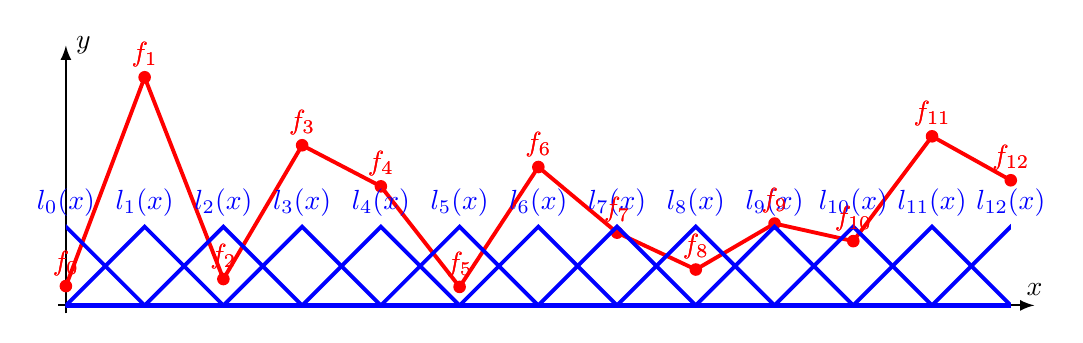
\begin{tikzpicture}[>=latex,thick]
\draw[->] (-0.1,0)--(12.3,0) coordinate[label={$x$}];
\draw[->] (0,-0.1)--(0,3.3) coordinate[label={right:$y$}];
\fill[color=red] (0,0.24529) circle[radius=0.08];
\fill[color=red] (1,2.89709) circle[radius=0.08];
\fill[color=red] (2,0.33458) circle[radius=0.08];
\fill[color=red] (3,2.03356) circle[radius=0.08];
\fill[color=red] (4,1.51182) circle[radius=0.08];
\fill[color=red] (5,0.23471) circle[radius=0.08];
\fill[color=red] (6,1.75737) circle[radius=0.08];
\fill[color=red] (7,0.92365) circle[radius=0.08];
\fill[color=red] (8,0.45537) circle[radius=0.08];
\fill[color=red] (9,1.03938) circle[radius=0.08];
\fill[color=red] (10,0.81606) circle[radius=0.08];
\fill[color=red] (11,2.14725) circle[radius=0.08];
\fill[color=red] (12,1.58882) circle[radius=0.08];

\uncover<1>{
\node[color=red] at (0,0.24529) [above] {$f_0$};
\node[color=red] at (1,2.89709) [above] {$f_1$};
\node[color=red] at (2,0.33458) [above] {$f_2$};
\node[color=red] at (3,2.03356) [above] {$f_3$};
\node[color=red] at (4,1.51182) [above] {$f_4$};
\node[color=red] at (5,0.23471) [above] {$f_5$};
\node[color=red] at (6,1.75737) [above] {$f_6$};
\node[color=red] at (7,0.92365) [above] {$f_7$};
\node[color=red] at (8,0.45537) [above] {$f_8$};
\node[color=red] at (9,1.03938) [above] {$f_9$};
\node[color=red] at (10,0.81606) [above] {$f_{10}$};
\node[color=red] at (11,2.14725) [above] {$f_{11}$};
\node[color=red] at (12,1.58882) [above] {$f_{12}$};
}

\draw[color=red,line width=1.4pt] 
   (0,0.24529) --
   (1,2.89709) --
   (2,0.33458) --
   (3,2.03356) --
   (4,1.51182) --
   (5,0.23471) --
   (6,1.75737) --
   (7,0.92365) --
   (8,0.45537) --
   (9,1.03938) --
   (10,0.81606) --
   (11,2.14725) --
   (12,1.58882);

\def\lfunktion#1{
\begin{scope}
	\clip (0,-0.1) rectangle (12,2);
	\draw[color=blue,line width=1.4pt]
		(-2,0)--({(#1)-1},0)--({(#1)},1)--({(#1)+1},0)--(13,0);
\end{scope}
	\node[color=blue] at ({#1},1) [above] {$l_{#1}(x)$};
}

\uncover<3>{\lfunktion{0}}
\uncover<4>{\lfunktion{1}}
\uncover<5>{\lfunktion{2}}
\uncover<6>{\lfunktion{3}}
\uncover<7>{\lfunktion{4}}
\uncover<8>{\lfunktion{5}}
\uncover<9>{\lfunktion{6}}
\uncover<10>{\lfunktion{7}}
\uncover<11>{\lfunktion{8}}
\uncover<12>{\lfunktion{9}}
\uncover<13>{\lfunktion{10}}
\uncover<14>{\lfunktion{11}}
\uncover<15>{\lfunktion{12}}

\uncover<3>{\node[color=red] at (0,0.24529) [above] {$f_0$};}
\uncover<4>{\node[color=red] at (1,2.89709) [above] {$f_1$};}
\uncover<5>{\node[color=red] at (2,0.33458) [above] {$f_2$};}
\uncover<6>{\node[color=red] at (3,2.03356) [above] {$f_3$};}
\uncover<7>{\node[color=red] at (4,1.51182) [above] {$f_4$};}
\uncover<8>{\node[color=red] at (5,0.23471) [above] {$f_5$};}
\uncover<9>{\node[color=red] at (6,1.75737) [above] {$f_6$};}
\uncover<10>{\node[color=red] at (7,0.92365) [above] {$f_7$};}
\uncover<11>{\node[color=red] at (8,0.45537) [above] {$f_8$};}
\uncover<12>{\node[color=red] at (9,1.03938) [above] {$f_9$};}
\uncover<13>{\node[color=red] at (10,0.81606) [above] {$f_{10}$};}
\uncover<14>{\node[color=red] at (11,2.14725) [above] {$f_{11}$};}
\uncover<15>{\node[color=red] at (12,1.58882) [above] {$f_{12}$};}

\end{tikzpicture}
\end{center}
\end{frame}
